\documentclass[12pt,a4paper]{report}
\usepackage[utf8]{inputenc}
\usepackage{amsmath}
\usepackage{amsfonts}
\usepackage{amssymb}
\usepackage{graphicx}
\usepackage{float}
\input defs.tex
\bibliographystyle{alpha}
\graphicspath{ {./figures/} }

\title{Game Theoretic Solutions to Power Control in MIMO Communications Systems}
\author{Peter Hartig}

\begin{document}
\maketitle

%\begin{abstract}
%This work investigate resource allocation strategies for such systems and in particular, those strategies minimizing system overhead. 
%\end{abstract}
%
%\newpage
\tableofcontents
\newpage

\chapter{Introduction}
\section{Introduction}
Modern communication systems often incorporate numerous, uncoordinated users competing for a limited resource.
In this work, a game theoretic approach considers a wireless communications network with uncoordinated  macrocell and femtocell users. The goal of this approach is to find Nash Equilibrium in which femtocell base stations optimize their utility while ensuring macrocell user interference is below a given threshold. 
Previous work has shown solutions for systems in which the femtocell base stations transmit over a SISO channel; therefore the MIMO case is investigated here. 
One of the primary goals of this work is to achieve Nash Equilibrium (NE) via distributed solutions which minimize system overhead. As seen in the following, the most general setup of this game does not permit such solutions and therefore a refined problem is proposed. Numerical results to the derived solution are then discussed. 


\section{Relevant Tools/Theory}

It is useful to first review relevant tools for solving such games. Together, these tools provide a series of steps to follow in solving for Nash Equilibrium via a distributed solution. 

\begin{enumerate}
\item The Concave N-Person game: a framework for proving existence and uniqueness of NE.

\begin{itemize}
\item
\textbf{Definition:} A game in which individual players maximize a concave utility function and the strategy set resulting from problem constraints (potentially player coupled) is convex. 
\item 
\textbf{Existence of Nash Equilibrium:} Pure Strategy NE exist for Concave N-Person  games \cite[Thm1]{rosen1964existence}. 
\item
\textbf{Uniqueness of Nash Equilibrium:} To prove uniqueness of NE for Concave N-Person  games, the "Normalized Nash Equilibrium" is introduced.
First, take a weighted sum of the player utility functions $U_{\mathrm{f}}(b)$.
\begin{equation}
\sigma(\mathbf{u},\mathbf{r})  = \Sigma_{\mathrm{f=1}}^{\mathrm{F}} r_{\mathrm{f}}U_{\mathrm{f}}(b),\; \mathbf{r}=(r_{\text{1}}... r_{\text{F}})
,\; \mathbf{u}=(u_{\text{1}}... u_{\text{F}})
, \; 
r_{\mathrm{f}} \geq 0
\end{equation}
 The function $G(b,r) $ is defined as the Jacobian of $g(b,r) $, with 
\begin{equation}
g(b,r)= 
\begin{bmatrix}
r_1 \nabla U_{1}(b)
\\
r_2 \nabla U_{2}(b)
\\
\vdots\\
r_F \nabla U_{F}(b)
\end{bmatrix}
\end{equation}


Negative Definiteness of the matrix $[G(b,r)+G^{T}(b,r)] $ is a sufficient condition for Diagonally Strict Concavity of $\sigma(u,r)$ which is a sufficient condition for uniqueness of a NNE \cite[Thm4]{rosen1964existence}


\end{itemize}
\item The Potential Function: representing the game using a single, central optimization problem.
\begin{itemize}
\item
\textbf{Definition:}  a function
$ \Psi(b_{\text{f}})$ which satisfies:
\begin{equation}\label{potential_game_condition}
\frac{\partial \Psi(b_{\text{f}})}{\partial b_{\text{f}}}
 =
 \frac{\partial U_(b_{\text{f}})}{\partial b_{\text{f}}}
\end{equation} 
for a game with player utility functions $U_(b_{\text{f}})$.
In words, $ \Psi(b_{\text{f}})$ is a function whose gradient with respect to the strategy $b_{\text{f}}$ of a player, is equal to the gradient of that player's utility function with respect to strategy $b_{\text{f}}$.
\item \textbf{Result:} Global optima to the potential function of a game are Nash Equilibrium.
\item \textbf{Convex Case:} If a Concave N-Person game admits a potential function, the potential function will be concave allowing for use of convex optimization tools to find a NE. 
\item \textbf{Additional Note:}  $ \Psi() $ is unique (A constant term can be added etc.)
\end{itemize}



\item Distributed Optimization: algorithms which solve a central optimization problem with multiple processes in parallel. 
\begin{itemize}
\item \textbf{Steps in Distribution:} 
\begin{itemize}
\item Begin with a central optimization problem (In this case obtained using a Potential Function to the game).
\item Determine the dual problem to the central, primal problem.
\item Evaluate if problem can be separated into sub-problems each with independent optimization variables.
\item Perform an ascent of the dual problem by iterating between solving the dual function of the sub-problems, then broadcasting these solutions to perform the gradient step of the dual problem.
\item In the case of strong duality to the problem, the dual ascent will converge to the optimal (In this case a Nash Equilibrium).

\end{itemize} 
\item \textbf{Benefit:} In the communications context, distribution of the optimization problem can reduce that amount of information that needs to be passed between different users of the communication network. 
\end{itemize}
\item Concave Programming: To discuss if needed for general setup


\end{enumerate}




\section{Outline}
Look at how the tools described above will be used in the work. 
\begin{itemize}
\item 
\ref{genmodel}: Introduces the system model for the most general setup of the game.
\item 
\ref{genproblem}: Analyze the general setup to see why further refinements are useful in arriving at a distributed solution. 
\item
\ref{conmodel}: Introduce refinements to the system model 
\item 
\ref{conproblem}: Solve the game using the refined system model
\item 
\ref{numerical}: Discuss numerical results to proposed solutions. 
\end{itemize}
\chapter{System Model}

\section{General System Model}\label{genmodel}

\subsection{Players: Femtocell Base Stations}


Each player of the game, a femtocell base station (FC-BS) $f \in \{1 ... F\}$ , is characterized by:
\begin{itemize}
\item 
$T_f$ antennas with which to transmit to $K_f$ femtocell users (it is assumed that $T_f \geq K_f$).
\\
\item 
	Beamforming matrix $\mathbf{U}_{\mathrm{f}} \in \mathbb{C}_{T_f \times K_f}$ such that the transmitted 		
	signal is $\mathbf{s}_{\mathrm{f}
	}= \mathbf{U_{\mathrm{f}}}\mathbf{x_{\mathrm{f}}}$. The 		
	vector of symbols for users of FC-BS $f$, $\mathbf{x_{\mathrm{f}}}$ is  normalized such that $E[\|\mathbf{x}_{\mathrm{f,i}}
	\|_2^2]=1$ and $E[\mathbf{x}_{\mathrm{f}}\mathbf{x}_{\mathrm{f}}^H]=\mathbf{I}$.
\\
\item 
	Power constraint $trace(\mathbf{U}_f^H\mathbf{U}_f) \leq P^{Total}_{f} $.

\item 
	Cost function $U_f() =
	\sum_{\mathrm{i=1}}^{\mathrm{K_f}}
    	 U_{\mathrm{f,i}}(\gamma_{\mathrm{f,i}}) $
    	in which all $U_{\mathrm{f,i}}()$ are non-decreasing (No assumption about concavity is made at this point).

\item 
	Knowledge of the downlink channel matrix $\mathbf{H_\mathrm{f}} \in \mathbb{C}_{K_f \times T_f} $ to the $K_f$ FC-BS users.
% TODO(Simulate degradation with incomplete CSI solution?)
\\
\item
	 FC-BSs are assumed to be spaced far apart in distance such that FC-BS $f$ 
	 causes no interference to the users of any other FC-BS. As a result, $U_f()$ is independent of other FC-BSs.
\end{itemize}

\subsection{Macrocell Users}
Macrocell users $m \in \{1 ... M\}$ introduce constraints into the game. These users are characterized by:

\begin{itemize}
\item 
	Received interference and constraint
	$\sum^F_{f=1} \mathbf{\tilde{h}}_{\mathrm{m,f}}^T  \mathbf{U_{\mathrm{f}}} 						
	\mathbf{U_{\mathrm{f}}^{\mathrm{H}}} \mathbf{\tilde{h}_{\mathrm{m,f}}^*} \leq I^{Threshold}		
	_{\mathrm{m}} $.

\item 
	FC-BS $f$ is assumed to know the downlink channel matrix $\tilde{\mathbf{H}_{\mathrm{f}}} \in \mathbb{C}_{M \times T_f}$ to all $M$ Macrocells users.
\\
\end{itemize}

\subsection{Femtocell Users}
\begin{itemize}

\item User $i$ of FC-BS $f$ has signal to interference plus noise ratio (SINR):
	\begin{equation*}
	\gamma_{\mathrm{f,i}} = \frac{\|\mathbf{h^H_{\mathrm{f,i}}u_{\mathrm{f,i}}}\|^2}
	{\sigma^2_{noise}   +
	\underbrace{
	 \sum_{\mathrm{\tilde{f}}=1,\mathrm{\tilde{f}}\neq f}^{\mathrm{F}} \sum_{\mathrm{u=1}}^{K_{\mathrm{\tilde{f}}}}
	\|\mathbf{h^H_{\mathrm{\tilde{f},u}}u_{\mathrm{\tilde{f},i}}}\|^2}_{\mathrm{inter-cell}}
	 + 
	 \underbrace{
	 \sum_{\mathrm{\tilde{k}\neq i}}^{\mathrm{K_f}}
	 \|\mathbf{h^H_{\mathrm{f,\tilde{k}}}u_{\mathrm{f,\tilde{k}}}}\|^2}_{\mathrm{intra-cell}}}
	  \; \mathrm{i \in \{1 ... K_f\}}\end{equation*}
\\
with AWGN $\sim \mathcal{CN}(0,\sigma^2_n)$
\\

By the sufficient spacing assumption above, this reduces to:
	\begin{equation*}
	\gamma_{\mathrm{f,i}} = \frac{\|\mathbf{h^H_{\mathrm{f,i}}u_{\mathrm{f,i}}}\|^2}
	{\sigma^2_{noise} 
	 + \sum_{\mathrm{\tilde{k}\neq i}}^{\mathrm{K_f}}
	  \|\mathbf{h^H_{\mathrm{f,\tilde{k}}}u_{\mathrm{f,\tilde{k}}}}\|^2}
	  \; \mathrm{i \in \{1 ... K_f\}}
	\end{equation*}
\\


\end{itemize}





\subsection{General Optimization Problem}\label{genproblem}

Each player $f$ attempts to maximize utility function $U_f()$ while satisfying the interference constraints imposed by the macro cell users and a transmission power constraint. 
\par




	\begin{subequations}
	\label{optim}
	\begin{align}
	    \underset{\mathbf{U}_{\mathrm{f}} }{\text{argmin}} \;
	    & - \sum_{\mathrm{i=1}}^{\mathrm{K_f}}
    	U_{\mathrm{f,i}}(\gamma_{\mathrm{f,i}}) \label{player_opt} \\
	    \text{subject to} \; &
	   \sum^F_{f=1} \mathbf{\tilde{h}}_{\mathrm{m,f}}^T  \mathbf{U_{\mathrm{f}}}		
	\mathbf{U_{\mathrm{f}}^{\mathrm{H}}} \mathbf{\tilde{h}_{\mathrm{m,f}}^*} \leq I^{Threshold}		
	_{\mathrm{m}} & m \in \{1 ...M\} 
		\label{interference_const_gen}\\
        & trace(\mathbf{U}_{\text{f}}^H\mathbf{U}_{\text{f}}) \leq P^{Total}_{\text{f}} \label{power_const_gen}\\
        & \langle \mathbf{h_{\text{f,j}}}\mathbf{u_{\text{f,i}}} \rangle =0\ & \; \forall j \in \{1... K_f\}\backslash i ,\; \forall i \in \{1 ... K_f\} \label{zf_const_gen}
	\end{align}
	\end{subequations}
	
In order to ensure the resulting game admits a potential function, constraint \eqref{zf_const_gen} restricts $\mathbf{U}_{\mathrm{f}}$ to the set of zero-forcing beamformers by.	
	
\subsection{Concave N-Person game analysis of general setup}
The convexity of the resulting problem is analyzed to investigate if this system permits the Concave N-Person game framework. 

\begin{enumerate}


\item
The constraints form a convex, closed and bounded set. 

\begin{itemize}

\item
	Constaint \eqref{interference_const_gen} contains $M$ quadratic constraints on $\mathbf{U_f}$ and 
	can be rewritten as 

\begin{gather*}
	\sum_{f=1}^F
	trace(\mathbf{U_f^H} \mathbf{\tilde{h}_{m,f}} \mathbf{\tilde{h}_{m,f}^H} \mathbf{U_f} )\leq 
	I^{Threshold}_{m}.
\end{gather*}
This can be further decomposed into  
	\begin{gather*}
	\sum_{f=1}^F
	\sum_{i=1}^{f_i}
	\mathbf{u_{\mathrm{f,i}}^H}\mathbf{\tilde{h}_{\mathrm{m,f}}} \mathbf{\tilde{h}}_{\mathrm{m,f}}^H
	\mathbf{u_{\mathrm{f,i}}} \leq I^{Threshold}_{m}
	\end{gather*}
in which the term $ \mathbf{\tilde{h}_{\mathrm{m,f}}} \mathbf{\tilde{h}}_{\mathrm{m,f}}^H$ is  a positive semi-definite matrix resulting in a convex set 
\cite[p.8,9]{BoV:04}. 
%This is essentially high dimensional ellipsoid.


\item \
	Constraint \eqref{power_const_gen} can be similarly decomposed into the sum
	\begin{gather*}
		\sum_{i=1}^{K_f}\mathbf{u_{\mathrm{f,i}}^{\mathrm{H}}} \mathbf{I} 		
		\mathbf{u_{\mathrm{f,i}}} \leq  P^{Total}_{f}
	\end{gather*}
	in which $\mathbf{I}$ is positive definite and 			
	therefore the constraint is strictly convex for the same 		
	reason as \eqref{interference_const_gen}.

\item 
	Constaint \eqref{zf_const_gen} is an affine constraint. 
		\begin{gather*}
		\langle \mathbf{h_{\mathrm{f,j}}}\mathbf{u_{\mathrm{f,i}}} \rangle =0
		\end{gather*}
%Note that affine constaints to not have to satisfy Slater's condition
\end{itemize}


\item Concavity of the utility function
\begin{itemize}
\item 
Due to the zero-forcing constraint \eqref{zf_const_gen}, $\gamma_{\mathrm{f,i}}$ becomes
	\begin{equation}\label{zf_snr}
	\gamma_{\mathrm{f,i}} = \frac{\|\mathbf{h^H_{\mathrm{f,i}}u_{\mathrm{f,i}}}\|^2}
	{\sigma^2_{noise}  
	}
	= 
	\frac{\mathbf{u^H_{\mathrm{f,i}}h_{\mathrm{f,i}}h^H_{\mathrm{f,i}}u_{\mathrm{f,i}}}}
	{\sigma^2_{noise}  
	}
	\end{equation}
	As $\mathbf{h}_{\mathrm{f,i}}\mathbf{h}^H_{\mathrm{f,i}}$ is positive semi-definite, $\gamma_{\mathrm{f,i}}$ is convex in ${\mathbf{u}_{\mathrm{f,i}}}$. 
\item
The composition $U_{\mathrm{f,i}}(\gamma_{\mathrm{f,i}}) $ is concave only if $U_{\mathrm{f,i}}() $ is concave and non-increasing; violating the non-decreasing definition of $U_{\mathrm{f,i}}() $.
If $U_{\mathrm{f,i}}() $ is a general, non-decreasing function, the result is quasiconvex \cite[p.~102]{BoV:04}. If $U_{\mathrm{f,i}}() $ is  non-decreasing and convex, the resulting
   function is convex and therefore, concave programming can be used to find a \emph{maximum}. 
\end{itemize}

\end{enumerate}

\subsection{Potential Game for General Problem}
Under the current system model, the game is not a Concave N-Person game. Nevertheless, because of the independence of the utility functions due to the spacing assumption, the game will still admit a potential function.


\section{Concave System Model}\label{conmodel}

The general setup of this game seen in the previous section prohibits the use of tools we wish to use in reaching a NE of the game.
The following refinement of the system model permits a unique Nash Equilibrium to be found via a single convex problem which may be distributed across players of the game.
\par
Rather than jointly optimizing the power allocation over the set of possible zero-forcing beamformers as in the general setup, the zero-forcing beamformer is pre-selected independently \emph{before} the allocation of power. 

\subsection{Players: Femtocell Base Stations}
Femtocells are adapted from the general setup to the refined setup:
\begin{itemize}
\item 
	FC-BSs with multiple antennas ($T_f \geq 1$) can beamform their transmission using the precoding 	
	matrix $\mathbf{U}_{\mathrm{f}} \in \mathbb{C}_{T_f \times K_f}$ .
	The columns of $\mathbf{U}_{\mathrm{f}}$ are now \emph{normalized} such that 
	 $\|\mathbf{u}_{\mathrm{fi}}\|^2 =1 \;\forall i \in \{1 ... K_f\}$.
\\

\item 
$\mathbf{U}_f$ is selected as a pseudo-inverse to $\mathbf{H_\mathrm{f}}$.
Such that
\begin{gather*}
\langle \mathbf{h_{f,j}}\mathbf{u_{f,i}} \rangle =0\  \; \forall j \in \{1... K_f\}\backslash i ,\; \forall i \in \{1 ... K_f\}
\end{gather*}. Later, choices for $\mathbf{U}_f$ will be considered for when there are additional degrees of freedom in the system (i.e when $T_{\text{f}}> K_{\text{f}}$.)

\item  
	FC-BS $f$ allocates  transmission power using the diagonal, power allocation  	
	matrix $\mathrm{diag}(\mathbf{p}_{\mathrm{f}})$ with $p_{\mathrm{fi}} \geq 0, \forall i \in \{1 ... K_f\}$
such that the transmitted 		
	signal is 
	$\mathbf{s}_{\mathrm{f}	}= \mathbf{U_{\mathrm{f}}} 
	\mathrm{diag}(\mathbf{p}_{\mathrm{f}})^{\frac{1}{2}}
	\mathbf{x_{\mathrm{f}}}$.
\\
\item 
	FC-BS $f$ enforces power constraint:
	\begin{gather*}
	trace(E[\mathbf{s}_\mathrm{f}\mathbf{s}_\mathrm{f}^H]) =
	\sum_{\mathrm{i=1}}^{\mathrm{K_{\mathrm{f}}}} p_{\mathrm{fi}}
	  \leq P^{Total}_{f} 
	  	\end{gather*}

% TODO(Simulate degradation with incomplete CSI solution?)


\item 
	Cost function $U_f() =
	\sum_{\mathrm{i=1}}^{\mathrm{K_f}}
    	U_{\mathrm{f,i}}(\gamma_{\mathrm{f,i}}) $
    	in which all $U_{\mathrm{f,i}}()$ are non-decreasing and
    	\emph{strictly concave}.
\item The SINR of the Femto Cell users is now
\begin{equation}\label{zf_snr}
	\gamma_{\mathrm{f,i}} = 	\frac{\mathbf{u^H_{\mathrm{f,i}}h_{\mathrm{f,i}}h^H_{\mathrm{f,i}}u_{\mathrm{f,i}}}}
	{\sigma^2_{noise}  
	}=\frac{\sum_{\mathrm{i=i}}^{\mathrm{K_{f}}}
 p_{\mathrm{fi}}\|h_{\mathrm{f,i}}u_{\mathrm{f,i}}\|^2}
	{\sigma^2_{noise}  
	}
	\end{equation}

\end{itemize}

\subsection{Macro Cell Users}
No change from general setup.

\subsection{Femtocell Users}
No change from general setup.



\subsection{Optimization Problem of player $f$}\label{conproblem}


	\begin{subequations}
	\label{optim}
	\begin{align}
	    \underset{\mathbf{p}_{\mathrm{f}} }{\text{minimize}} \;
	    & - \sum_{\mathrm{i=1}}^{\mathrm{K_f}}
    	U_{\mathrm{f,i}}(p_{\mathrm{f,i}}) \label{player_opt_c} \\
	    \text{subject to} \; &
	  \sum^F_{f=1} \mathbf{\tilde{h}}_{\mathrm{m,f}}^T  \mathbf{s}_{\mathrm{f}} 						
	\mathbf{s_{\mathrm{f}}^{\mathrm{H}}} \mathbf{\tilde{h}_{\mathrm{m,f}}^*} 
	=
	\sum_{\mathrm{f=1}}^{\mathrm{F}}	\sum_{\mathrm{i=1}}^{\mathrm{K_f}}
	p_{\mathrm{f,i}}\|\tilde{h}_{\mathrm{m,f}}^T u_{\mathrm{f,i}}\|^2_2
	\leq I^{Threshold}		
	_{\mathrm{m}} & m \in \{1 ...M\} 
		\label{interference_const_c}\\
        & trace(\mathbf{s}_\mathrm{f}\mathbf{s}_\mathrm{f}^H) =
        	\sum_{\mathrm{i=1}}^{\mathrm{K_{\mathrm{f}}}} p_{\mathrm{f,i}}
	   \leq P^{Total}_{f}  \label{power_const_c}\\
        & p_{\mathrm{f,i}} \geq 0 &  i \in \{1 ...K_{\mathrm{f}}\} \label{pos_power_const_c}
	\end{align}
	\end{subequations}

Note that because $\mathbf{U}_{\mathrm{f}}$ is pre-selected as a pseudo-inverse to  $\mathbf{H_\mathrm{f}}$, constraint \eqref{zf_const_gen} has been removed.

\subsection{Concave N-Person game analysis of concave setup}

Sufficient conditions for a concave problem are:

\begin{enumerate}

\item
The constraints form a convex, closed and bounded set. 

\begin{itemize}

\item
	Constaint \eqref{interference_const_c} contains $M$ affine constraints on $diag(\mathbf{p_{\mathrm{f}}})$.

\begin{gather*}
	  \sum^F_{f=1} \mathbf{\tilde{h}}_{\mathrm{m,f}}^T  \mathbf{s}_{\mathrm{f}} 						
	\mathbf{s_{\mathrm{f}}^{\mathrm{H}}} \mathbf{\tilde{h}_{\mathrm{m,f}}^*} 
	=
	\sum_{\mathrm{f=1}}^{\mathrm{F}}	\sum_{\mathrm{i=1}}^{\mathrm{K_f}}
	p_{\mathrm{fi}}\|\tilde{h}_{\mathrm{mf}}^T u_{\mathrm{f,i}}\|
	\leq I^{Threshold}_{\mathrm{m}} 
\end{gather*}

\item \
	Constraint \eqref{power_const_c} is  affine in $diag(\mathbf{p_{\mathrm{f}}})$.
	
\item \
	Constraint \eqref{pos_power_const_c} is affine in $diag(\mathbf{p_{\mathrm{f}}})$.
\end{itemize}

%Note that affine constaints to not have to satisfy Slater's condition

\item The utility function is assumed concave in its argument $p_{\mathrm{f,i}}$.

\end{enumerate}

This problem satisfies the conditions for the Concave N-Persion game and therefore a pure strategy Nash Equilibrium exists due to 
\cite[Thm1]{rosen1964existence}.

As the utility function $U_{\mathrm{fi}}(p_{\mathrm{fi}})$ is strictly concave, (differentiable?), and independent of all $p_{\mathrm{fj}}$ the matrix $[G(b,r)+G^{T}(b,r)] $ is diagonal with values on the diagonal $<0$. As $[G(b,r)+G^{T}(b,r)] $ is negative definite the Normalized Nash Equilibrium are unique \cite[Thm4]{rosen1964existence}.

\subsection{Potential Game for Concave Problem}

\textbf{Potential Function:} The proposed potential function satisfying \eqref{potential_game_condition} is 

\begin{gather*} \label{Potential_Function}
\Psi(\mathbf{\gamma}) = \sum_{f = 1}^{F} U_f(\mathbf{\gamma_{\mathrm{f}}}) 
\end{gather*}

resulting in the single optimization problem 
	
		\begin{subequations}
	\label{optim}
	\begin{align}
	    \underset{\mathbf{p}}{\text{minimize}}
	    & \; \Psi(\mathbf{\gamma}) \label{potential_game} \\
	    \text{subject to} \; &
	  \sum^F_{f=1} \mathbf{\tilde{h}}_{\mathrm{m,f}}^T  \mathbf{s}_{\mathrm{f}} 						
	\mathbf{s_{\mathrm{f}}^{\mathrm{H}}} \mathbf{\tilde{h}_{\mathrm{m,f}}^*} \leq I^{Threshold}		
	_{\mathrm{m}} & m \in \{1 ...M\} 
		\label{interference_const}\\
        & trace(\mathbf{s}_\mathrm{f}\mathbf{s}_\mathrm{f}^H)  \leq P^{Total}_{f}  \label{power_const}
        & \forall f \in \{1 ... F\}\\
        & p_{\mathrm{f,i}} \geq 0 &  \forall i \in \{1 ...K_{\mathrm{f}}\} \; \forall f \in \{1 ... F\}\label{pos_power_const}
	\end{align}
	\end{subequations}
	with $\mathbf{\gamma}= [\mathbf{\gamma_{\mathrm{1}}},\mathbf{\gamma_{\mathrm{2}}}...\mathbf{\gamma_{\mathrm{F}}}]$

%\begin{theorem}\label{distributed}
%\cite{ghosh2015normalized}
%If a game's potential function is strictly concave and the derivative of the function with respect to the individual players variables are independent of the other player variables, then there exists a distributed solution.
%\end{theorem}

\subsection{Distributed Solution to the Game}
A distribtued solution to \eqref{potential_game} is now proposed.
\subsubsection{Central Problem Resulting from Potential Game}
The Lagrangian to the potential function is derived to formulate the dual problem. 
\begin{multline}
L(\mathbf{U,\lambda}) = 
\;
\sum_{f=1}^F U_f(\gamma_{\text{f}}) 
+
\sum_{\mathrm{m=1}}^M \lambda_{\mathrm{m}}
(	  \sum^F_{f=1} \mathbf{\tilde{h}}_{\mathrm{m,f}}^T  \mathbf{s}_{\mathrm{f}} 						
	\mathbf{s_{\mathrm{f}}^{\mathrm{H}}} \mathbf{\tilde{h}_{\mathrm{m,f}}^*} - I^{Threshold}		
	_{\mathrm{m}} )
\\
+ 
\sum_{f=1}^F
\chi_{\mathrm{f}}(trace(\mathbf{s}_\mathrm{f}\mathbf{s}_\mathrm{f}^H)-P^{Total}_{f} )
+
\sum_{f=1}^F 
\sum_{i=1}^{K_f}
\nu_{\mathrm{f,i}}(-p_{\mathrm{f,i}})
\end{multline}

The corresponding dual function is
\begin{gather*}
g(\lambda,\nu) = \underset{\mathbf{p}}{\mathrm{argmin}}\;L(\mathbf{U,\lambda})
\end{gather*}
and the resulting dual problem is
\begin{gather*}
\underset{\lambda}{\mathrm{argmax}}\;\underset{\mathbf{p}}{\mathrm{argmin}}\;L(\mathbf{U,\lambda}) = \underset{\lambda}{\mathrm{argmax}}\;g(\lambda,\nu)
\end{gather*}

This dual function can be decomposed into $F$ component functions


\begin{multline}
g_f(\lambda,\nu) = \underset{\mathbf{p_f}}{\mathrm{argmin}}
\{
\;
U_f(\gamma_{\text{f}}) 
+
\sum_{\mathrm{m=1}}^M \lambda_{\mathrm{m}}
(\mathbf{\tilde{h}}_{\mathrm{m,f}}^T  \mathbf{s}_{\mathrm{f}} 						
	\mathbf{s_{\mathrm{f}}^{\mathrm{H}}} \mathbf{\tilde{h}_{\mathrm{m,f}}^*} - \frac{I^{Threshold}_{\mathrm{m}}}{F})
\\
+ 
\chi_{\mathrm{f}}(trace(\mathbf{s}_\mathrm{f}\mathbf{s}_\mathrm{f}^H)-P^{Total}_{f} )
+
\sum_{i=1}^{K_f}
\nu_{\mathrm{f,i}}(-p_{\mathrm{f,i}})\}
\end{multline}
\\

The problem can now be solved using a distributed dual ascent to reach the NE of the potential game. 
\subsubsection{Distributed Algorithm 1}\label{algo1}
In the following algorithms and simulation results $U_{\text{f}}(\gamma_{\text{f}}) = log(1+\gamma_{\text{f}})$.

\begin{enumerate}
\item 
Individual players (FC-BSs) can solve $ g_f(\lambda,\nu) $ independently.
\begin{itemize}
\item Setting $\frac{\partial g_f(\lambda,\nu)}{\partial p_{\mathrm{f,i}}} = 0$ 
and solving for $p_{\mathrm{fi}}$ using \eqref{zf_snr} yields

\begin{gather}
p_{\mathrm{fi}} = (\sum_{\mathrm{m=1}}^{\mathrm{M}}\lambda_{\mathrm{m}}\|\mathbf{\tilde{h}}_{m,f}^T \mathbf{u}_{\mathrm{f,i}}\|^2_2
+\chi_{f} \|\mathbf{u}_{\mathrm{f,i}}\|^2_2
-\nu_{\mathrm{f,i}}
 )^{-1}
  - \sigma^2_n
\end{gather}

\end{itemize}
\item 
Using $g(\lambda,\nu) = \sum_{f=1}^{F}g_f(\lambda,\nu)$ and rules from subgradient calculus 
$\partial g(\lambda,\nu) = \sum_{f=1}^{F} \partial g_f(\lambda,\nu)$ 
, the dual variables can updated with:

\begin{gather}
\lambda_{\mathrm{m}}^{\mathrm{k+1}} = (
\lambda_{\mathrm{m}}^{\mathrm{k}}
+
\alpha^{\mathrm{k}}*
(
\underbrace{
\sum _{\mathrm{f=1}}^{\mathrm{F}}
\sum _{\mathrm{i=1}}^{\mathrm{K_{\mathrm{f}}}}
p_{\mathrm{fi}}
\|\mathbf{\tilde{h}}_{\mathrm{mf}}^T \mathbf{u_{\mathrm{fi}}}\|^2_2}_{Interference}
- I_{\mathrm{m}}
))^+
\end{gather}
performed at the macro cell users,

\begin{gather}
\chi_{\mathrm{f}}^{\mathrm{k+1}} = (
\chi_{\mathrm{f}}^{\mathrm{k}}
+
\alpha^{\mathrm{k}}*
(\underbrace{\sum_{\mathrm{i=1}}^{\mathrm{K_{\mathrm{f}}}} p_{\mathrm{fi}}}_{Used Power} - P_{\mathrm{f}}^{Total}) )^+
\end{gather}
performed at individual FC-BSs, and 

\begin{gather}
\nu_{\mathrm{fi}}^{\mathrm{k+1}} = (
\nu_{\mathrm{fi}}^{\mathrm{k}}
+
\alpha^{\mathrm{k}}*
(-p_{\mathrm{fi}}))^+
\end{gather}
also performed at individual FC-BSs.
As each of dual variables in this update is an inequality constraint, the implementation of this algorithm directly enforces non-negativity using 
$(arg)^+$.
Step size $\alpha^{\mathrm{k}}$ is predefined and constant.
 % must satisfy  $\sum_{\mathrm{k=1}}^{\infty} \alpha^{\mathrm{k}}$ (cite).



\end{enumerate} 
These local updates require require that additional information is passed through the system. In particular this requires that Macro Cell Users monitor their incoming interference and then broadcast the updated dual variable $\lambda_{\text{m}}$ with which FC-BSs update the power allocation. 
Note also that the dual ascent algorithm uses the dual and thus cannot guarantee a feasible solution to the primal problem originally posed. (Discuss constraint tolerance used here? )

\subsection{Beamformer Optimization for Convex Setup}
When additional degrees of freedom are available in choosing $\mathbf{U}_{\mathrm{f}}$ after satisfying the zero-forcing constraint (i.e. $T_{\text{f}}> K_{\text{f}}$ ), these degrees of freedom may be utilized to optimize an objective function of the FC-BS choosing the beamformer. 
The first objective function is that which minimizes the noise enhancement and corresponds to the Moore-Penrose pseudoinverse (CITE). 
    \begin{equation}
    \begin{array}{ll}
    \underset{\mathbf{U}_{\mathrm{f}} }{\text{argmin}}   & tr(\sigma_n\mathbf{U_{\mathrm{f}}}  \mathbf{U_{\mathrm{f}}}^H)
    \\
    \mbox{subject to} & \mathbf{H}_{\mathrm{f}}^T  \mathbf{U_{\mathrm{f}}} = \mathbf{I}
    \end{array}
    \label{e-opt-prob}
    \end{equation}

Next, we consider the objective function which would minimize the correlation of the chosen beamformer with the known macro cell user channels.

    \begin{equation}
    \begin{array}{ll}
    \underset{\mathbf{U}_{\mathrm{f}} }{\text{argmin}}   & \sum^F_{f=1} \|\mathbf{\tilde{H}}_{\mathrm{f}}^T  \mathbf{U_{\mathrm{f}}}\|^2
    \\
    \mbox{subject to} & \mathbf{H}_{\mathrm{f}}^T  \mathbf{U_{\mathrm{f}}} = \mathbf{I}
    \end{array}
    \label{e-opt-prob}
    \end{equation}
This is problem convex in $\mathbf{U}_{\mathrm{f}}$ and can be found easily at individual FC-BSs (See if Largrangian yields analytic solution?).
We also consider the a problem in which FC-BS minimize correlation with macro cell users while also maximize correlation with channels of its own users. 
    \begin{equation}
    \begin{array}{ll}
    \underset{\mathbf{U}_{\mathrm{f}} }{\text{argmin}}   & \alpha\sum^F_{f=1} \|\mathbf{\tilde{H}}_{\mathrm{f}}^T  \mathbf{U_{\mathrm{f}}}\|^2
    -
    (1-\alpha)\sum^F_{f=1} \|\mathbf{H}_{\mathrm{f}}^T  \mathbf{U_{\mathrm{f}}}\|^2, \; 0\leq \alpha \leq 1
    \\
    \mbox{subject to} & \mathbf{H}_{\mathrm{f}}^T  \mathbf{U_{\mathrm{f}}} = \mathbf{I}
    \end{array}
    \label{e-opt-prob}
    \end{equation}
    This problem is not convex in $\mathbf{U}_{\mathrm{f}}$ thus we need to employ additional optimization techniques to find such $\mathbf{U}_{\mathrm{f}}$.
Note objective function of Moore-Penrose


\chapter{Simulation and Results}\label{numerical}
\subsection{Simulation System Description}
The Heterogeneous Network is simulated by randomly placing $F$ FC-BSs and $M$ Macro Cell Users within a predefined area. Each FC-BS is assigned $K_{\mathrm{f}}$ unique Femto Users. All channels between FC-BS and users (both Femtro and Macro) are simulated using rayleigh fading and attenuation coefficient $d^{- \beta}$ with $\beta =2$ and $d$ as the distance between user and base-station.
FC-BS $f$ initializes power to user $i$ as $p_{\mathrm{fi}} = \frac{P^{P_{\mathrm{f}}^{Total}}}{K_{\mathrm{f}}} $ such that the corresponding power constraint is not violated. 
Dual variables are initialized using  
\par
For the case in which the utility function is differentiable w.r.t all of the optimization parameters, this can effectively be seen as a coordinate ascent over a differentiable function(does this allow for any sort of asynchronous updating?). As a result, the $\alpha^{k}$ used to ascend the dual do not need to be the same for the three updates (CITE).
TODO show dual problem is differentiable.


\subsection{Simulation Results}
Using the algorithm in \ref{algo1}, convergence to a Nash Equilibrium is observed over different system scenarios. 
\subsubsection{Simulation Results for Concave Setup}

\begin{figure}[H]
	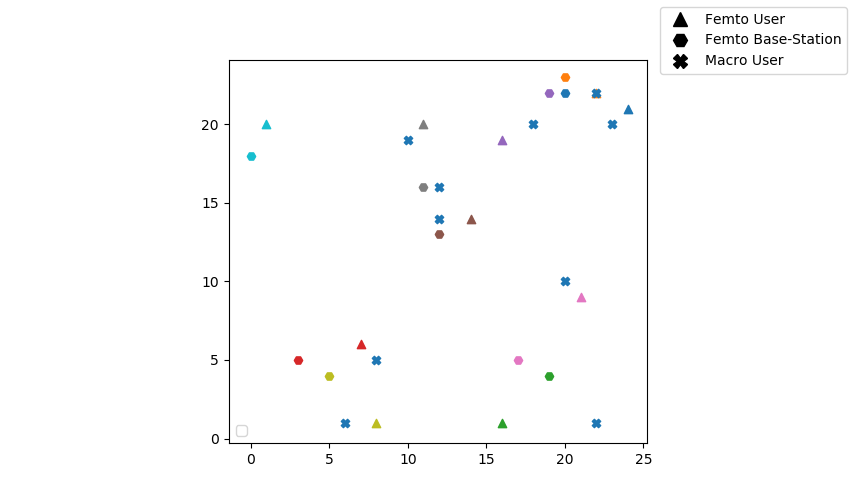
\includegraphics[width=\textwidth,height = 10cm]{figures/system_figure_single}
	  \caption{Simluation Setup Single Antenna and User.  }
\end{figure}

\begin{figure}[H]
	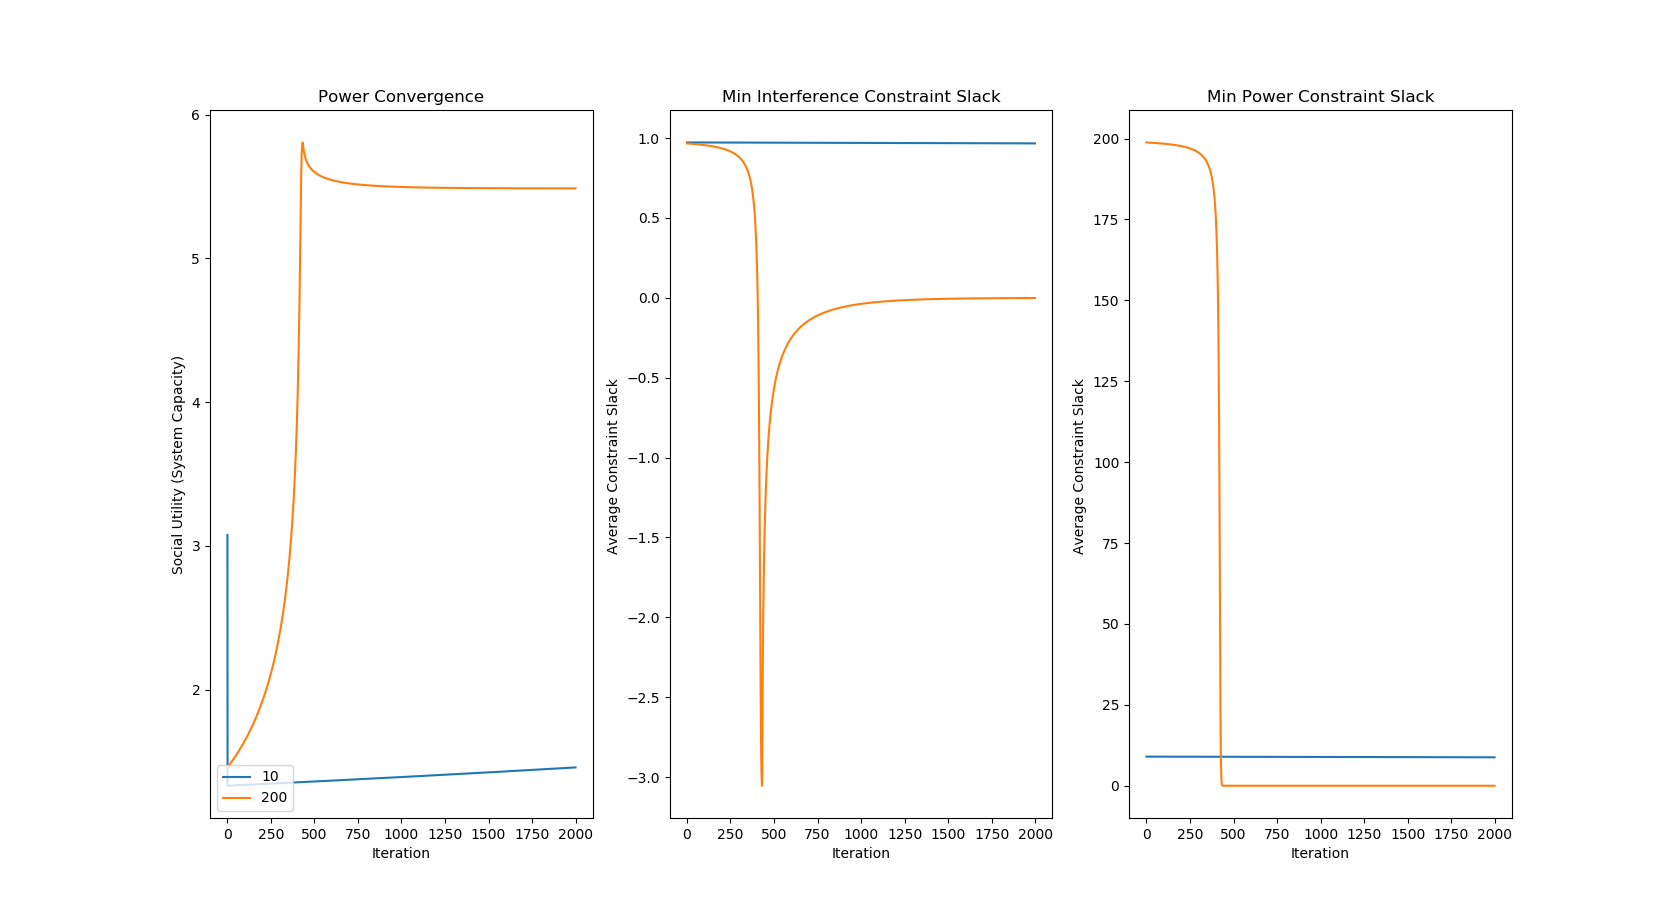
\includegraphics[width= 15cm,height = 10cm]{figures/single_power}
	  \caption{Single Antenna Game Simulation with different base station power constraints}
\end{figure}

\begin{figure}[H]
	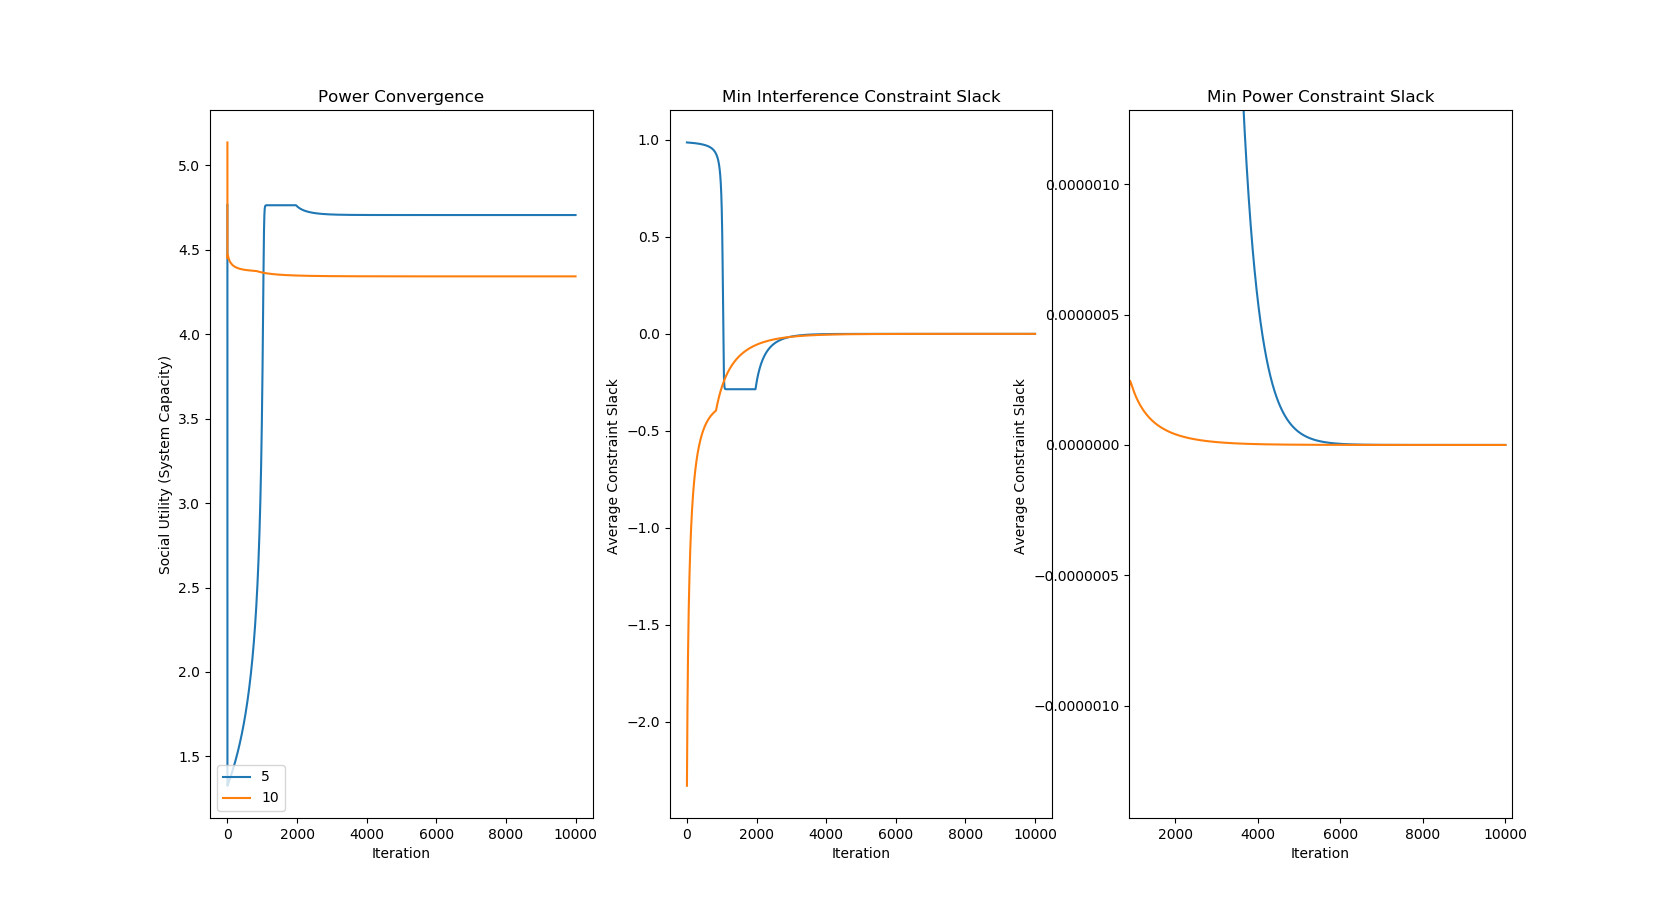
\includegraphics[width= 15cm,height = 10cm]{figures/single_macro}
	  \caption{Single Antenna Game Simulation with different numbers of macro cell users}
\end{figure}

\begin{figure}[H]
	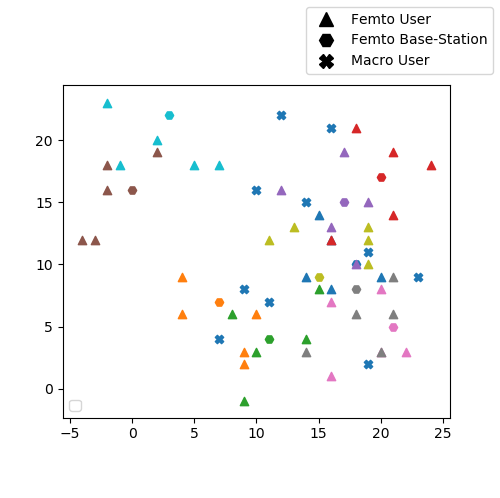
\includegraphics[width=\textwidth,height = 10cm]{figures/system_figure_multiple}
	  \caption{Simluation Setup Multiple Antenna and User.
	  }
\end{figure}


\begin{figure}[H]
	  	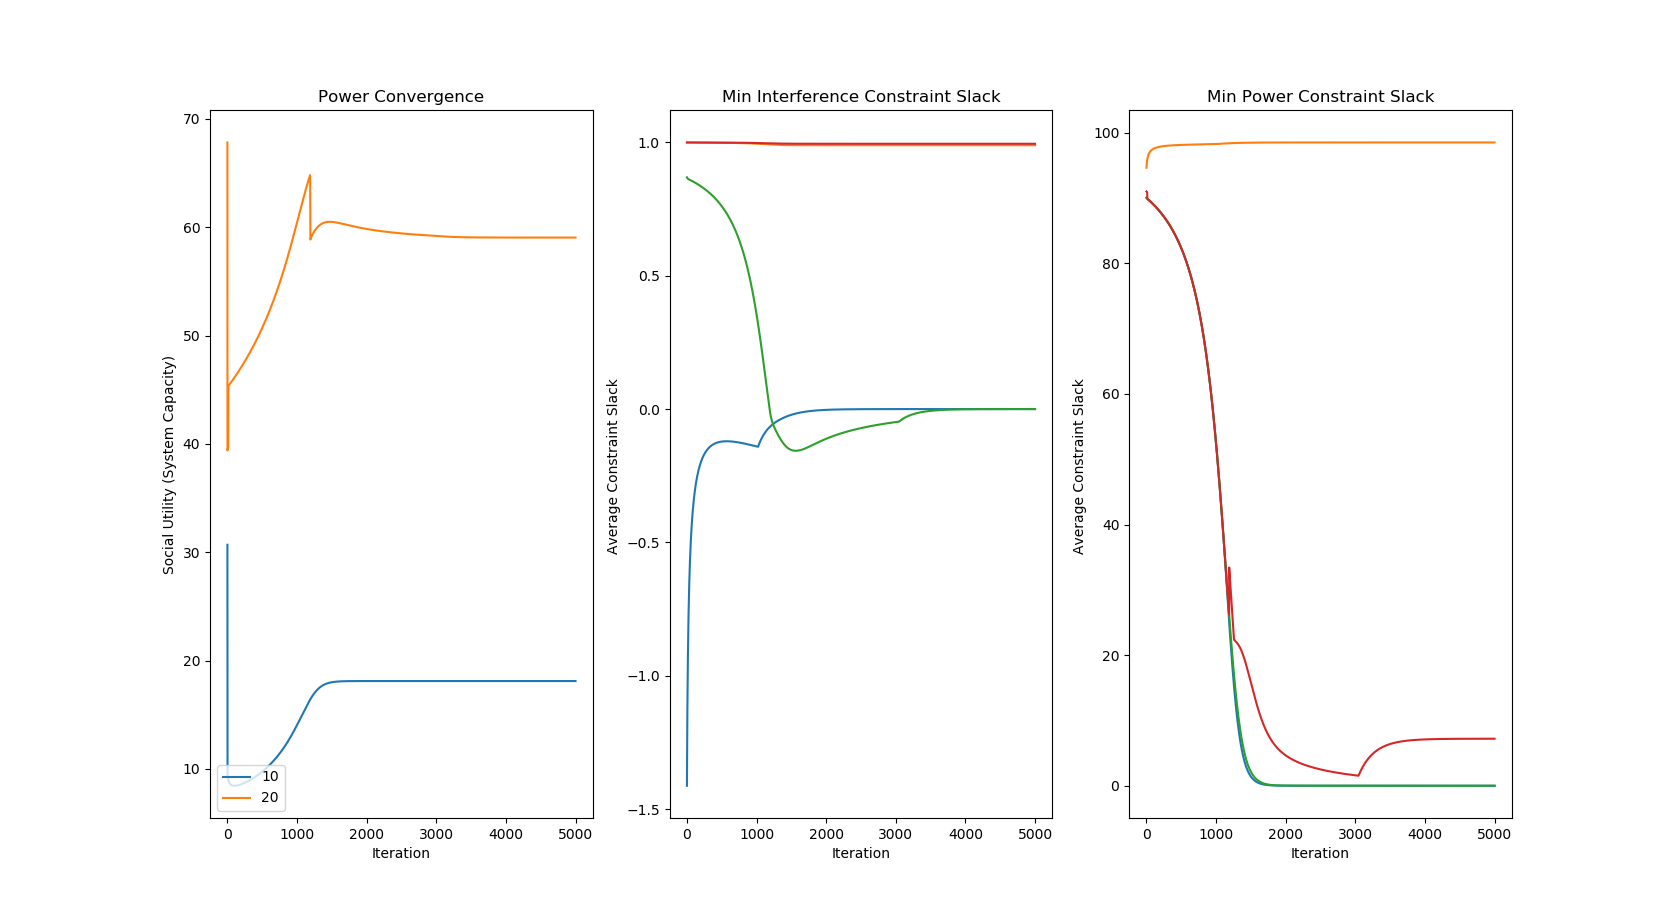
\includegraphics[width=\textwidth,height = 7cm]{figures/increasing_antenna}
	  		  \caption{Convergence for different numbers of antennas at FC-BSs. Number of femto cell users and macro cell users constant. Each BS has 10 users.}
	  \label{fig:}
\end{figure}


\begin{figure}[H]
	  	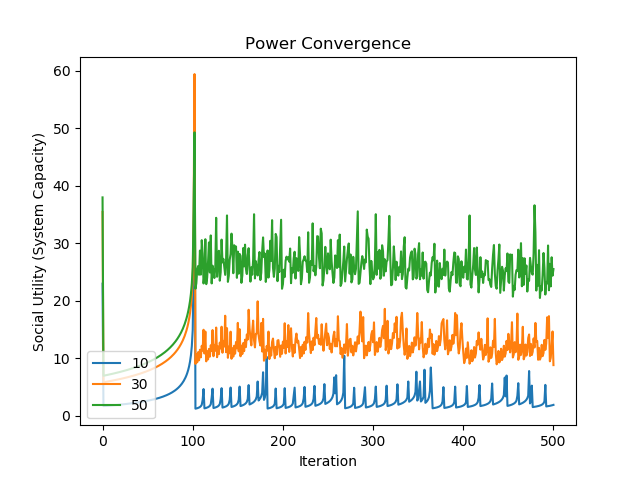
\includegraphics[width=\textwidth,height = 7cm]{figures/increasing_antenna_game_beamformer}
	  		  \caption{Different choices for the zero-forcing beamformer $\mathbf{U}_{\text{f}}$}
	  \label{fig:inc_fc}
\end{figure}

The concave setup of the FC-BS utility function is contingent upon knowledge of the channel state information $\mathbf{H}_{\text{f}}$. We now evaluate the effect of imperfect estimate of $\mathbf{H}_{\text{f}}$ on the solution. Imperfect CSi is simulated by adding additive white gaussian noise to the entries in $\mathbf{H}_{\text{f}}$. Need to check if this is even reasonable to simulate because might no longer be a game. 

\begin{figure}[H]
	  	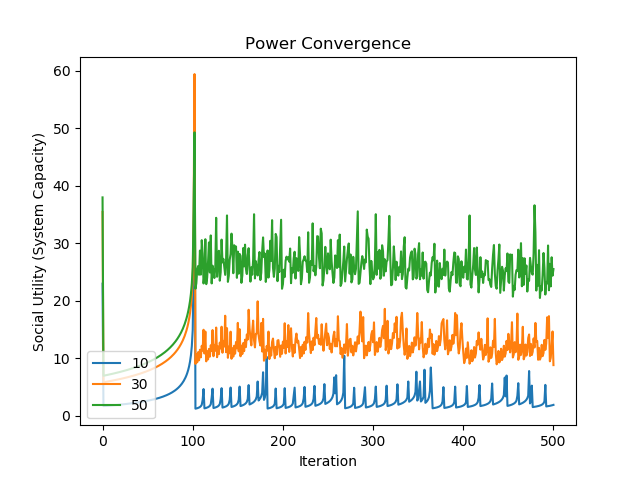
\includegraphics[width=\textwidth,height = 7cm]{figures/increasing_antenna_game_beamformer}
	  		  \caption{Impact of imperfect estimate of $\mathbf{H}_{\text{f}}$ at FC-BS $f$}
	  \label{fig:inc_fc}
\end{figure}


\chapter{Conclusion}

\newpage
\bibliography{gt_report}
\end{document}
